%
% Simple asymmetric two-column CV 
% Author: Sofia JIJON
%

\documentclass[a4paper,10pt]{article}
\usepackage[vmargin=1.5cm, hmargin=1.5cm]{geometry}
% !TEX root = Simple-CV.tex
%-------------------------------------------------------------------------------------------------------
% Packages
%-------------------------------------------------------------------------------------------------------
\usepackage[latin1]{inputenc}
\usepackage[T1]{fontenc}
\usepackage[english]{babel}
\usepackage{fontspec}
\defaultfontfeatures{
    Path = /usr/local/texlive/2021/texmf-dist/fonts/opentype/public/fontawesome/ }
\usepackage{fontawesome}
\usepackage{datetime}
\usepackage[usenames,dvipsnames]{xcolor}
\usepackage[colorlinks=true, urlcolor=ColorTwo]{hyperref}
\usepackage{tikz}
\usepackage{hyperref}
\usepackage{setspace}
\usepackage{graphicx}
\usepackage{enumitem}
\usepackage{sectsty}
\usepackage{multicol}
\usepackage{adjustbox}
%-------------------------------------------------------------------------------------------------------
% Layout
%-------------------------------------------------------------------------------------------------------
\pagenumbering{gobble}
\renewcommand{\baselinestretch}{1.5} 
\setlength{\parindent}{0pt}

%
% Color theme
%
\definecolor{ColorOne}{RGB}{0,110,140} 	% Blue
\definecolor{ColorTwo}{RGB}{120,0,120} 	% Mauve
%\definecolor{ColorTwo}{RGB}{140,100,0} 	% Gold

\sectionfont{\color{ColorOne}} 
\subsectionfont{\color{ColorOne}} 

%
% Vertical line
%
\newcommand{\MyVerticalRule}{%
	\textcolor{ColorOne}{\rule{1pt}{\textheight}}
}

%
% Update
%
\newcommand{\LastUpdate}{%
\vfill
\centering \small
\textcolor{ColorOne}{Last updated: \monthname,~\the\year.}
}

%
% Skip
%
\newcommand{\MySkip}{
\vskip12pt
}

%
% Format hyperrefs
%
\newcommand{\myhref}[2]{%
\href{#1}{\textcolor{ColorTwo}{#2}}
}
%
% Format skill bullets
%
\newcommand{\SkillBull}[1]{%
\textcolor{ColorTwo}{#1}
}


%-------------------------------------------------------------------------------------------------------

\begin{document}
\thispagestyle{empty}

%-------------------------------------------------------------------------------------------------------
% Left column
%-------------------------------------------------------------------------------------------------------
\begin{adjustbox}{valign=t}
\begin{minipage}{0.3\textwidth} % Adapt width to your convenience
%----------------------------------------------------
% Please add a photo in 1x1 format
\begin{center}
\begin{tikzpicture}
	\clip (0,0) circle (2cm) node {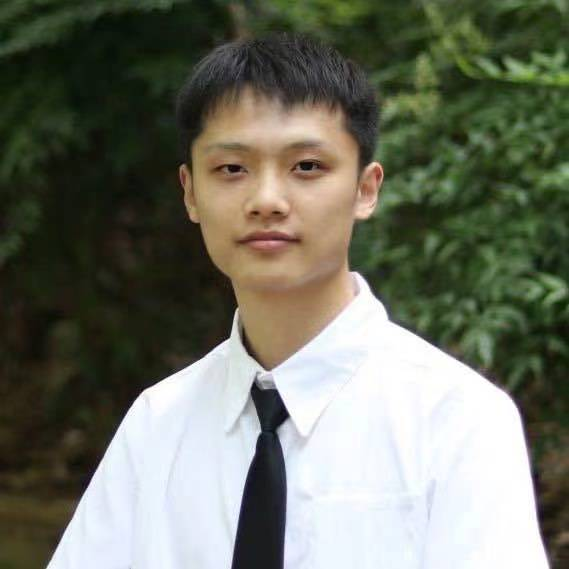
\includegraphics[width=4cm]{photo.jpg}};
\end{tikzpicture}

\MySkip 	% See MySetup.tex file

%----------------------------------------------------
{\LARGE \bfseries Wang Lei}

\MySkip 	% See MySetup.tex file

Born on Jan. 29th, 1999\\

Currently living in Beijing City\\

A first year postgraduate student @ UCAS, ICT

\MySkip 	% See MySetup.tex file

\textcolor{ColorTwo}{\faGithub} 
\myhref{https://github.com/LeiWang1999}{LeiWang1999} \\


\textcolor{ColorTwo}{\faChain} 
\myhref{https://leiblog.wang}{https://leiblog.wang} \\

\textcolor{ColorTwo}{\faEnvelopeO} 
\myhref{mailto:wanglei21c@mails.ucas.ac.cn}{wanglei21c@mails.ucas.ac.cn}

\end{center}

\vfill

%----------------------------------------------------
\section*{Scientific interests}
\raggedright
\textcolor{ColorOne}{$\circ$} Multi-Level IR \\
\textcolor{ColorOne}{$\circ$} Domain Specific Architecture \\
\textcolor{ColorOne}{$\circ$} Compiler Optimization\\
\textcolor{ColorOne}{$\circ$} DL Compiler

\vfill

%----------------------------------------------------
\section*{Education}
	\begin{description}
	\raggedright

	\item [\normalfont \textcolor{ColorOne}{Aug. 2021 - Present}] \textbf{Master in Computer Science}\\
	University of Chinese Academy of Science \\
	Institute of Computing Technology

	\item [\normalfont \textcolor{ColorOne}{Aug. 2017 - Jun. 2021}] \textbf{Bachelor in Electronic Engineering} \\ 
	Nanjing Tech University \\
	\textcolor{red}{Overall GPA:  3.95 / 4.00}
	\textcolor{red}{Ranking:  1 / 59}
	
\end{description}

\vfill
\end{minipage}
\end{adjustbox}
%
%
%-------------------------------------------------------------------------------------------------------
% Vertical rule
%-------------------------------------------------------------------------------------------------------
%
\hfill
\begin{adjustbox}{valign=t}
\begin{minipage}{0.05\textwidth} % Adapt width to your convenience
\MyVerticalRule  % See MySetup.tex file
\end{minipage}
\end{adjustbox}
\hfill
%
%-------------------------------------------------------------------------------------------------------
% Right column
%-------------------------------------------------------------------------------------------------------
\begin{adjustbox}{valign=t}
\begin{minipage}{0.6\textwidth} % Adapt width to your convienience
%----------------------------------------------------
\section*{Currently Situation}
\begin{description}
	\raggedright
	\item I'm currently a first year postgraduate student @ UCAS,ICT.\\
	My research interests lie in ML System and Optimization, looking for an internship opportunity helps me dive deeply into DL Compiler Stack. \\
	I enjoy writing post: \myhref{https://zhuanlan.zhihu.com/p/442140282}{MLIR: A Brief Survey}\\
	I'm also a contributor of \myhref{https://github.com/OAID/Tengine}{Tengine} and \myhref{https://github.com/buddy-compiler/buddy-mlir}{buddy-mlir}.

\end{description}

\section*{Awards \& Honor}
\begin{description}
\raggedright
\item [] \textbf{Competetion} \\
	First Price of 2019 National Undergraduate Electronics Design Contest \\
	Third prize of National FPGA Competition \\
	\myhref{https://leiblog.wang/about}{more competition awards.}
	\item [] \textbf{Scholarship} \\
	2018 Chinese National Scholarship $\left( Top 、 0.3 \% \right)$ \\
	2019 School Principle's Scholarship $\left( Top 、 0.1 \% \right)$ \\
	2020 School Principle's Scholarship $\left( Top 、 0.1 \% \right)$ \\
	First Prize Scholarship x 3 $\left( Top 、 3 \% \right)$ \\
	Special Prize Scholarship x 4 $\left( Top 、 3 \% \right)$ 


\end{description}

%----------------------------------------------------
\section*{Experience}
\begin{description}
\raggedright
\item[\normalfont \textcolor{ColorOne}{Sep. 2021 - Oct. 2021.}] 
	\textbf{Netease Intelligent Hardware R\&D Department}\\ \medskip
	
	NPU / DLA Development intern.\\
	
	NVDLA(Nvidia Deep Learning Accelerator, an opensource DLA) FPGA deployment and Software stack porting.
	
\end{description}

%----------------------------------------------------
\section*{Oral communications}
\begin{description}
	\raggedright
	\item [\normalfont \textcolor{ColorOne}{Sep. 23th, 2021.}] 
	\textbf{Tengine Open Talk : New Backend OpenDLA.} [\myhref{https://github.com/LeiWang1999/ZYNQ-NVDLA/blob/master/TengineTalk.pdf}{slides}] [\myhref{https://www.bilibili.com/video/BV1z44y1478k}{recording}]

	I made a big pull requst \myhref{https://github.com/OAID/Tengine/pull/1061}{\#1061} to integrate NVDLA with Tengine.
\end{description}


\MySkip

%----------------------------------------------------
\LastUpdate
%----------------------------------------------------
\end{minipage}
\end{adjustbox}
\end{document}
